\documentclass[times, twocolumn]{article}
\usepackage{graphicx} % Required for inserting images
\usepackage{subcaption}
\usepackage{amsmath}
\usepackage{float}
\usepackage{pgfplots}
\usepackage{subcaption}
\usepackage{comment}
\usepackage[a4paper, total={7in, 9in}]{geometry}
\usepackage{biblatex}

\addbibresource{mybib.bib}

\title{Spotify Tracks Genre Classification}
\author{Nabeha Barkatullah, Mia Striebeck, Laksha Karthikeyan, Carson Chiem, Shuzo Naruse}
\date{May 20, 2024}

\begin{document}
\maketitle

\newpage
% abstract
\begin{abstract}
Discovering new music that fits within your music taste is time-consuming and difficult. On top of there being an abundance of music to sift through, finding songs from the bulk that you actually enjoy listening to can go either way. With this project, we aim to utilize a Spotify dataset to build a model to classify songs under genres, with the potential of being part of a song recommendation system. Using the attributes from the dataset, such as the relevant music listening patterns and classification of songs, we will predict the genre a song falls under. Our goal is to build a classification model that predicts a song’s genre based on user-inputted track features.
\end{abstract}
\section{Introduction}
With music production becoming increasingly accessible, music platforms have subsequently become saturated with new music. For newer or more niche artists, being discovered among a sea of other songs and competing within the platform’s algorithm. On the other hand, for users looking for new music, breaking beneath the surface of more popular songs within genres they may enjoy can prove difficult and sifting through songs to curate their music profile can prove to be time consuming and frustrating when you are not exactly sure what you are looking for. 

This project is posed to be a part of a larger music recommendation system; this aspect of the system encompasses a machine learning driven genre classification model using the K-nearest neighbors method. To narrow down the scope of this project, we have our tool limited to music on Spotify’s platform for data feature accessibility— music uploaded to Spotify has an associated song ID, among other descriptive features about the song. Using Spotify music data sourced from Kaggle, a machine learning model based on K-nearest neighbors was trained and connected to the front end of a web based GUI.  In terms of the front end interaction, the user is able to navigate through our GUI which utilizes a Spotify API in order to input a song from search and predict the genre it belongs to. As a part of a larger product, this model would be used in tandem with other tools to fine tune a recommendation system based upon other aspects apart from the genre. 

For the task of genre classification, machine learning appeared to be the obvious approach due to the apparent degree of subjectivity of the task— the classification of a song into a genre is not always a clear choice but a decision can be made based upon patterns in music. ML is especially useful in this case where genre patterns can help form clearer decision boundaries. Additionally songs often do not belong to one single genre— more often than not they belong to multiple genres such as “Pop-Rock”, “Indie-Pop”, “Country-Blues”. With this in mind, utilizing K-nearest neighbors as an ML method provides a robust solution for the proposed task of genre classification as it provides a cluster of genres that most closely fit the inputted song. 

% background
\section{Background}
%literature review
\section{Literature Review}
Many previous works have utilized machine learning techniques to classify music by genre. R. Prajwal and Sharma et al. (2021) built multiple classification models based on features extracted from audio samples, such as spectral centroid (the weighted mean of the sound frequencies) and the shape of sound signals~\cite{Singhal2022}. They conducted feature selection and hyperparameter tuning using GridSearchCV and RandomizedSearchCV, optimizing the k value for k-NN to maximize accuracy~\cite{Singhal2022}. The models implemented included k-Nearest Neighbors (KNN), Support Vector Machine (SVM), Logistic Regression, and Random Forests~\cite{Singhal2022}. SVM achieved the highest accuracy of 76.4\%, followed by Random Forests with 69.6\%, KNN with 66.4\%, and Logistic Regression with 67.2\%, all after hyperparameter tuning~\cite{Singhal2022}.\\

While their dataset utilized technical audio features such as zero-crossing rate and mel-frequency cepstrum coefficients, our dataset includes numerical measures of musical elements and human interpretations of music, such as the mode, which describes the mood of a song. This is more similar to the work by Rahul Singhal and Shruti Srivatsan, who noted that classification models using Extreme Gradient Boosting and Random Forest performed the best compared to traditional ML approaches~\cite{prajwal2021music}. In particular, a hyperparameter-tuned Random Forest classifier achieved high accuracy and F1-score~\cite{prajwal2021music}.\\

Given that our dataset encompasses features like popularity, acousticness, and danceability, we wanted to explore how Random Forest would perform for our model. The KNN algorithm is noted for its simplicity in terms of workings and calculations. It offers flexibility for various modifications to overcome limitations, enhance accuracy, and increase its applicability to a wider variety of datasets. KNN's adaptability allows for performance improvements through optimizing the k parameter, refining distance calculations, and adding weights to different data points.

\section{Dataset Description and EDA}
\subsection{Dataset Description}
The original Kaggle dataset contains data on Spotify songs from over 125 genres, with each song having associated features related to identification of each track, audio characteristics, or popularity and genre classifications. The original set contained around 114k data points (songs/tracks) condensed in a CSV format, with 20 features, which are track id, artist name, album name, track name, popularity, duration (ms), explicit, danceability, energy, key, loudness, mode, speechiness, acousticness, instrumentalness, liveness, valence, tempo, and time signature. Popularity is the ranking of each song on a scale of 1 to 100, duration of the track is in milliseconds (ms), explicit is a boolean value, stating if a song contains explicit lyrics, danceability is a level, from 0 to 1, of a song being considered suitable for dancing, energy is a measure, from 0 to 1, of intensity, key is in regards to overall musical pitch, loudness is measured in decibels (dB), mode indicates if the track is on a major or minor scale (1 or 0), speechiness measures, from 0 to 1, the level of spoken words in a track, acousticness is a measure, from 0 to 1, of instruments used without electrical amplification, instrumentalness is a measure, from 0 to 1, of a track containing vocals, liveness is the likelihood of a song being performed in front of an audience, valence measures the interpretation of a song as positive or negative, tempo is the speed of a track, measured in beats per minute (BPM), and time signature indicates the number of beats in each measure of the piece. All are continuous variables, except for track id, artist name, album name, track name, explicit, popularity and track genre, which are categorical. Popularity is particularly ordinal categorical, as tracks are assigned a ranking of popularity. 

In pre-processing the data, we checked for duplicate rows and missing values. 32,656 rows were dropped, as they were each identified as having the same track name and artist as an another track. The remaining rows of distinct tracks were filtered to identify missing values for each feature, which identified one track having 3 missing values. Furthermore, the genre feature originally contained 125 classes, however, as many genres were more specific sub-genres, these sub-genres were grouped under their respective overall genres. For instance, tracks with the sub-genres "emo," "punk," and "garage," were all re-classified under the genre "punk-rock." This allowed for greater accuracy of genre classification, with reduced complexity and risk of overfitting, as the model would be less likely to fit too closely to the data of these more specific sub-genres, and a larger sample size within the overall genre would allow for greater accuracy. The dataset was ultimately filtered to only contain the 10 most popular genres, removing the rows of all other genres. Thus, the resulting cleaned dataset contained 81,344 rows of distinct tracks.

\subsection{Exploratory Data Analysis}
We conducted exploratory data analysis in order to further investigate the distributions of the features in our dataset and their correlations with each other, to identify potential presence of multicollinearity or irregularities, to help perform feature selection and identify the top 10 most frequent artists and genres in this dataset.

Figure \ref{graph:dists} shows frequency distributions of the features, showing that the danceability and tempo features have nearly normal distributions, while the distribution of loudness is left-skewed, and acousticness, speechiness, liveness are right-skewed. This signifies that while most of the songs in this dataset are moderately loud, there are some that have particularly low levels of loudness, that makes the distribution skew to the right. Similarly, acousticness, speechiness and liveness have similar levels among most of the songs, although there are some outlier songs with significantly higher levels of acousticness, speechiness and liveness that cause these distributions to skew to the right.

% adding Figure 1 - image of feature distributions
\begin{figure}[H]
    \centering
    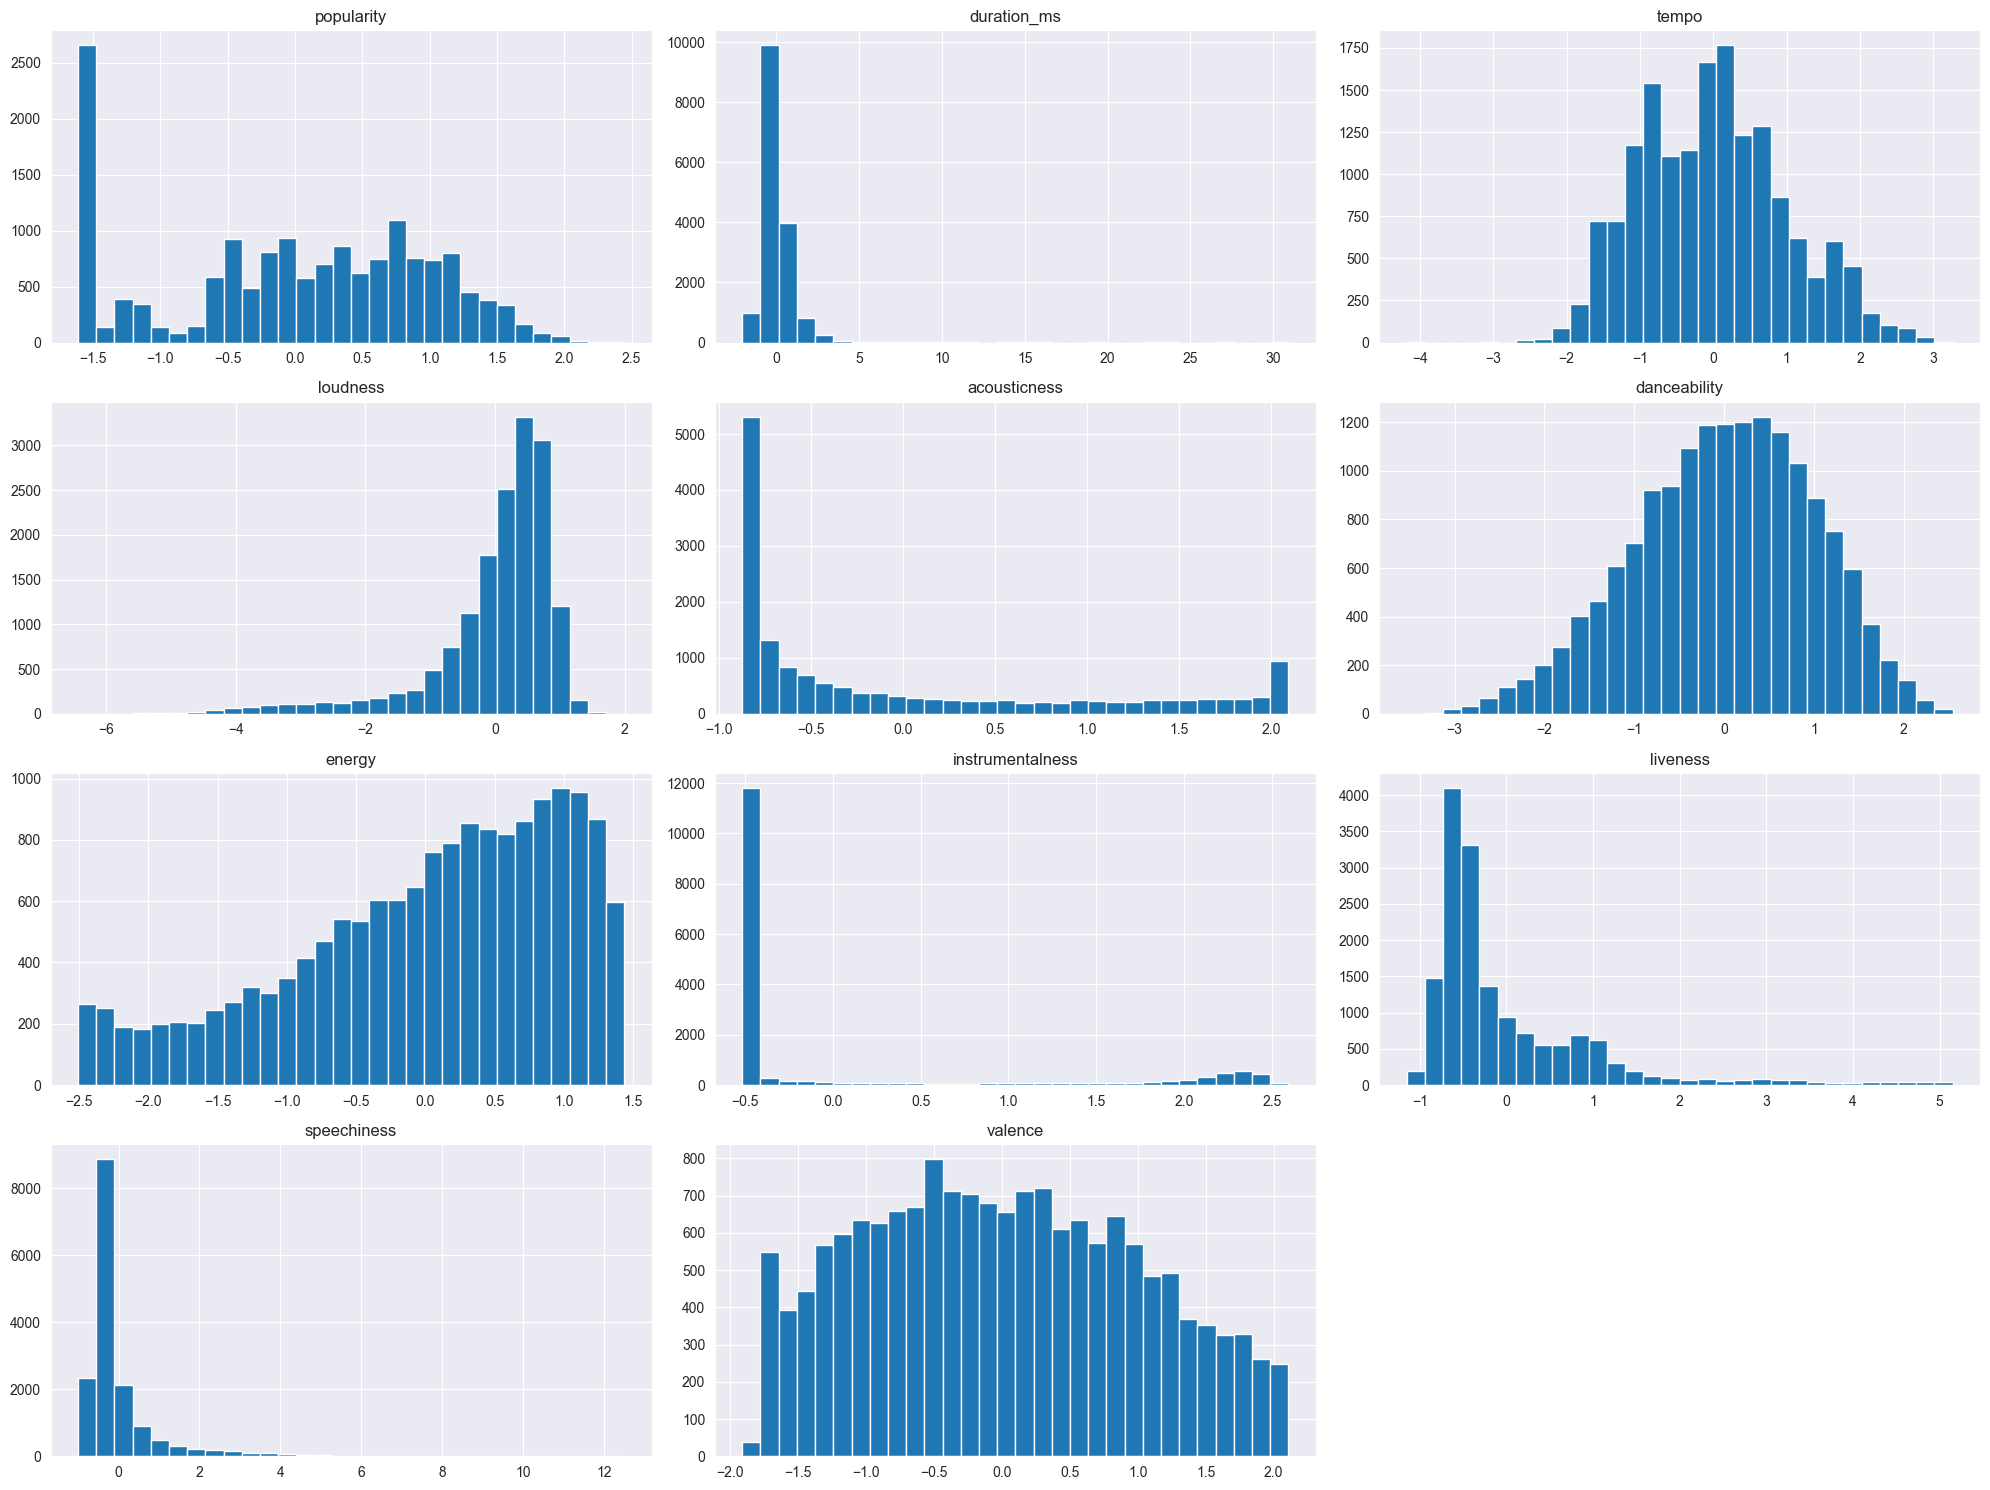
\includegraphics[width=0.55\textwidth]{feature_dists.png}
    \caption{Frequency distributions of the continuous track features, which have been scaled using z-score normalization.}
    \label{graph:dists}
\end{figure}

Box plots were used to further examine the distributions and identify outliers, as seen in Figure \ref{Boxplots}, which maps the distributions for the ordinal categorical predictor variable popularity, and every continuous predictor variable, which include duration, tempo, loudness, acousticness, danceability, energy, instrumentalness, liveness, speechiness and valence. From this visualization, it is evident that popularity, acousticness, energy and valence have no outliers, while all other features do, although it is expected that popularity contains no outliers, as these are ranked values of a pre-determined range. The presence of outliers is reasonable as it merely shows the diversity of the songs in our dataset, and ultimately, the variety in levels of these features is what characterizes the different music styles that allow a song to be categorized under a certain genre.
% adding Figure 2 - boxplots
\begin{figure}[H]
    \centering
    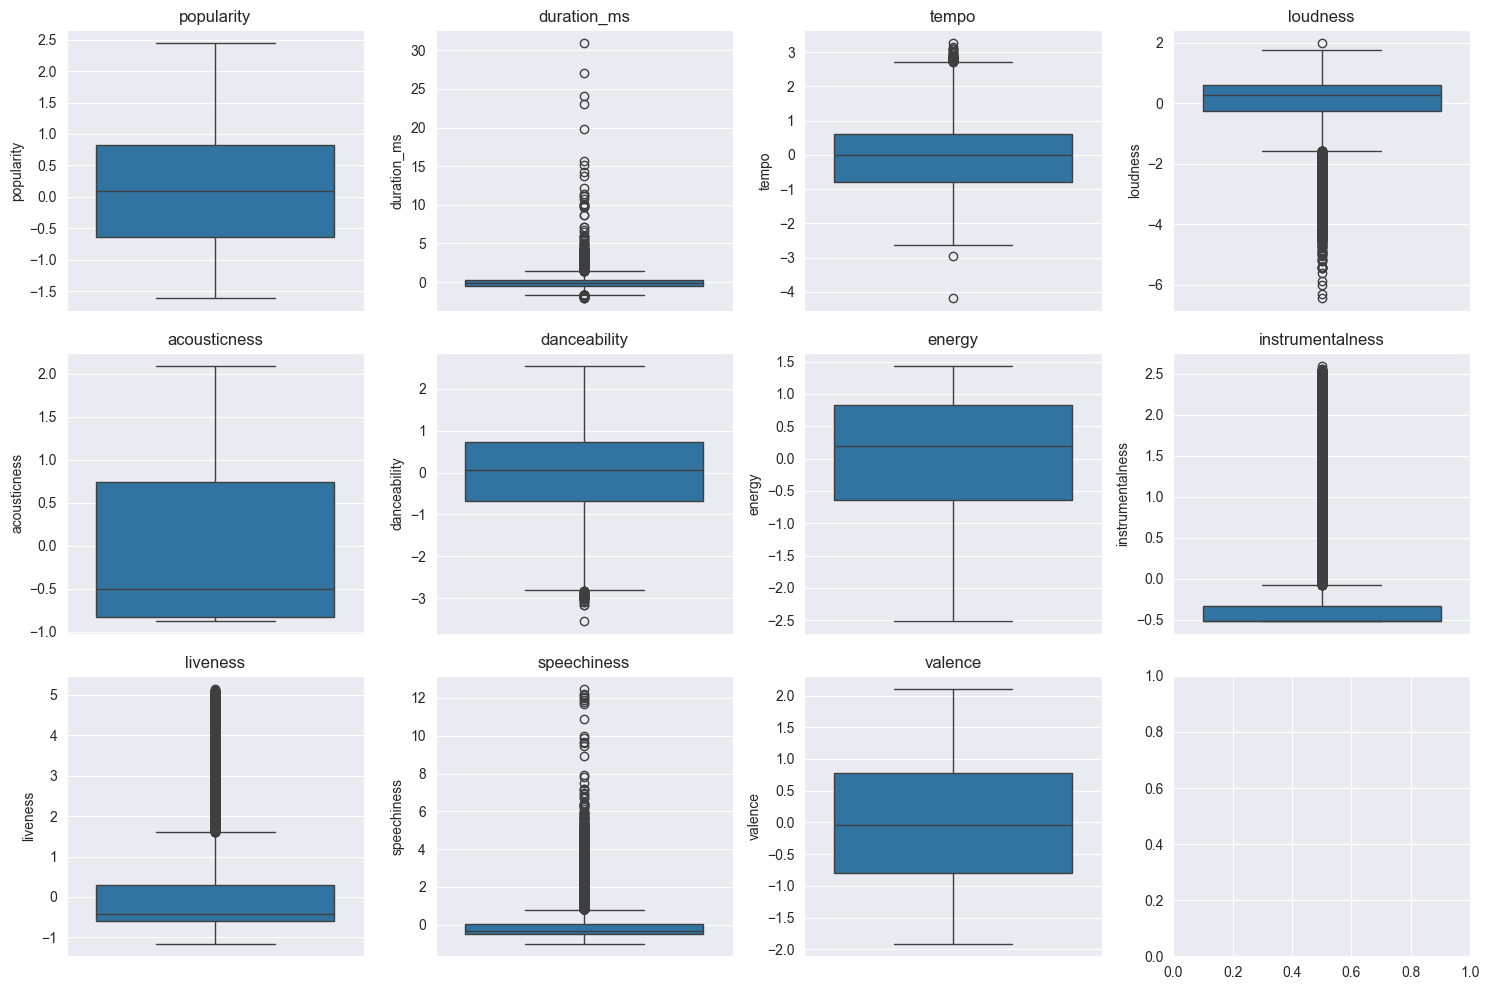
\includegraphics[width=0.5\textwidth, height=10cm]{feat_boxplots.png}
    \caption{Box plots depicting the distributions of the continuous features in our dataset, scaled using z-score normalization.}
    \label{Boxplots}
\end{figure}
Figure \ref{heatmap} displays the correlations between the continuous predictor variables in the dataset. It shows a significant positive correlation between energy and loudness, and that acousticness is significantly, negatively correlated with both loudness and energy. Further, danceability and valence appear to have a weak positive correlation, and instrumentalness and loudness have a weak negative correlation. Although the significant correlations between multiple features, such as between acousticness with loudness and energy, indicates multicollinearity, it is slight and therefore not likely to have a significant impact on the results of our classification model.
\begin{figure}[H]
    \centering
    \textbf{Pearson's Correlation Heatmap of Relevant Features}
    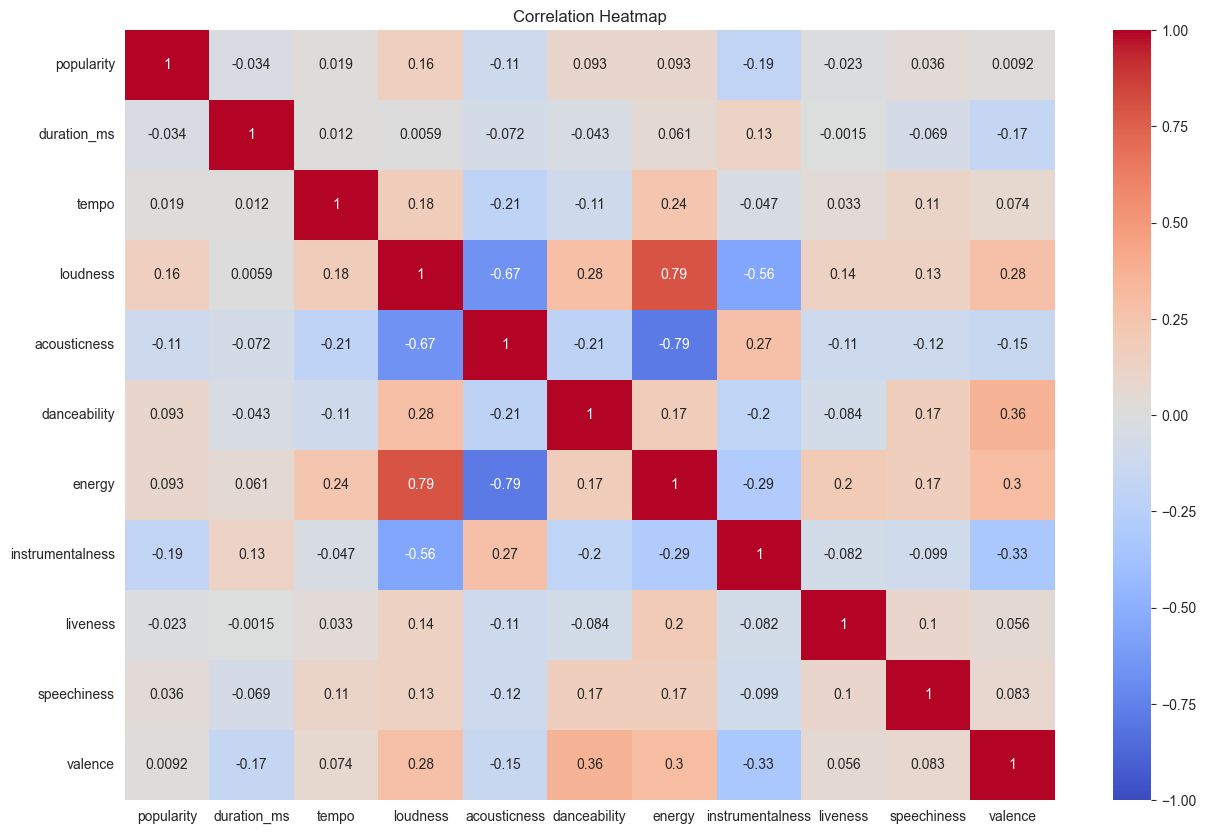
\includegraphics[width=1.0\linewidth]{corr_heatmap.png}
    \caption{The Pearson's correlation heatmap depicts the pairwise correlations between the 11  continuous features that are relevant to the characteristics of each track, where a value less than 0 indicates negative correlation, and a value greater than 0 indicates positive correlations between the features.}
    \label{heatmap}
\end{figure}

Figure \ref{top10} depicts the 10 most frequent artists and the top 10 most frequent genres that are present in the cleaned dataset. The 10 genres with the greatest frequency of tracks in this dataset are Electronic Dance Music (EDM), punk-rock, pop, rock, alt-rock, rock, acoustic, k-pop, classical, piano, and hip-hop. 

% adding Figure 4 - top 10 most frequent
\begin{figure}[H]
    \centering
    \includegraphics[width=0.5\textwidth]{top_10.png}
    \caption{Top 10 artists and genres}
    \label{top10}
\end{figure}

These results provided valuable insights into the distributions and spread of our individual features, as well as the varying frequency of tracks for all the different genres. This was useful information in choosing methods that would be best suitable for the characteristics of the dataset, and evaluating the performance of our models.

\section{Proposed Methodology}
In order to build a classification model to classify the genre of a track based on the predictor variables related to audio characteristics, our modeling approach entailed identifying techniques that would work well for multi-class classification, as our dataset contains multiple possible genres. We examined the performance of K-nearest neighbors clustering and Random Forest models.

\section{Experimental Results and Evaluation}
\subsection{Model Performances}

\subsection{Model Implications}

\section{Conclusion}

\section{Discussion}

\section{Github link and Project Roadmap}

\section{Works Cited}
\printbibliography


\end{document}
